\chapter{Figure and Table}

\graphicspath{ {graphics/Chapter4/} }

In a scientific document, it is necessary and essential to insert several figures or table to visualize the results.

\section{Insert Images}
	
	\LaTeX~provides several options to handle images and make them look exactly what you need. In this section, some basic operations are explained, e.g. how to include images, how to shrink or enlarge them and how to reference them within your document.
	
	The following code block shows a basic example to insert a figure into the text (see Figure \ref{fig_1}). The explanations for each line of code are also written in the code block. 
	
	\lstset
	{
		language=[LaTeX]TeX,
		breaklines=true,
		basicstyle=\ttfamily\scriptsize,
		keywordstyle=\color{blue},
		moretexcs={\includegraphics},
		xleftmargin=1cm,
		xrightmargin=1cm,
		aboveskip=0\baselineskip
	}

	\begin{lstlisting}
\begin{figure}[h!]
	% position the figure at the horizontal center
	\centering
	% figure width set to 0.8 times the width of text body
	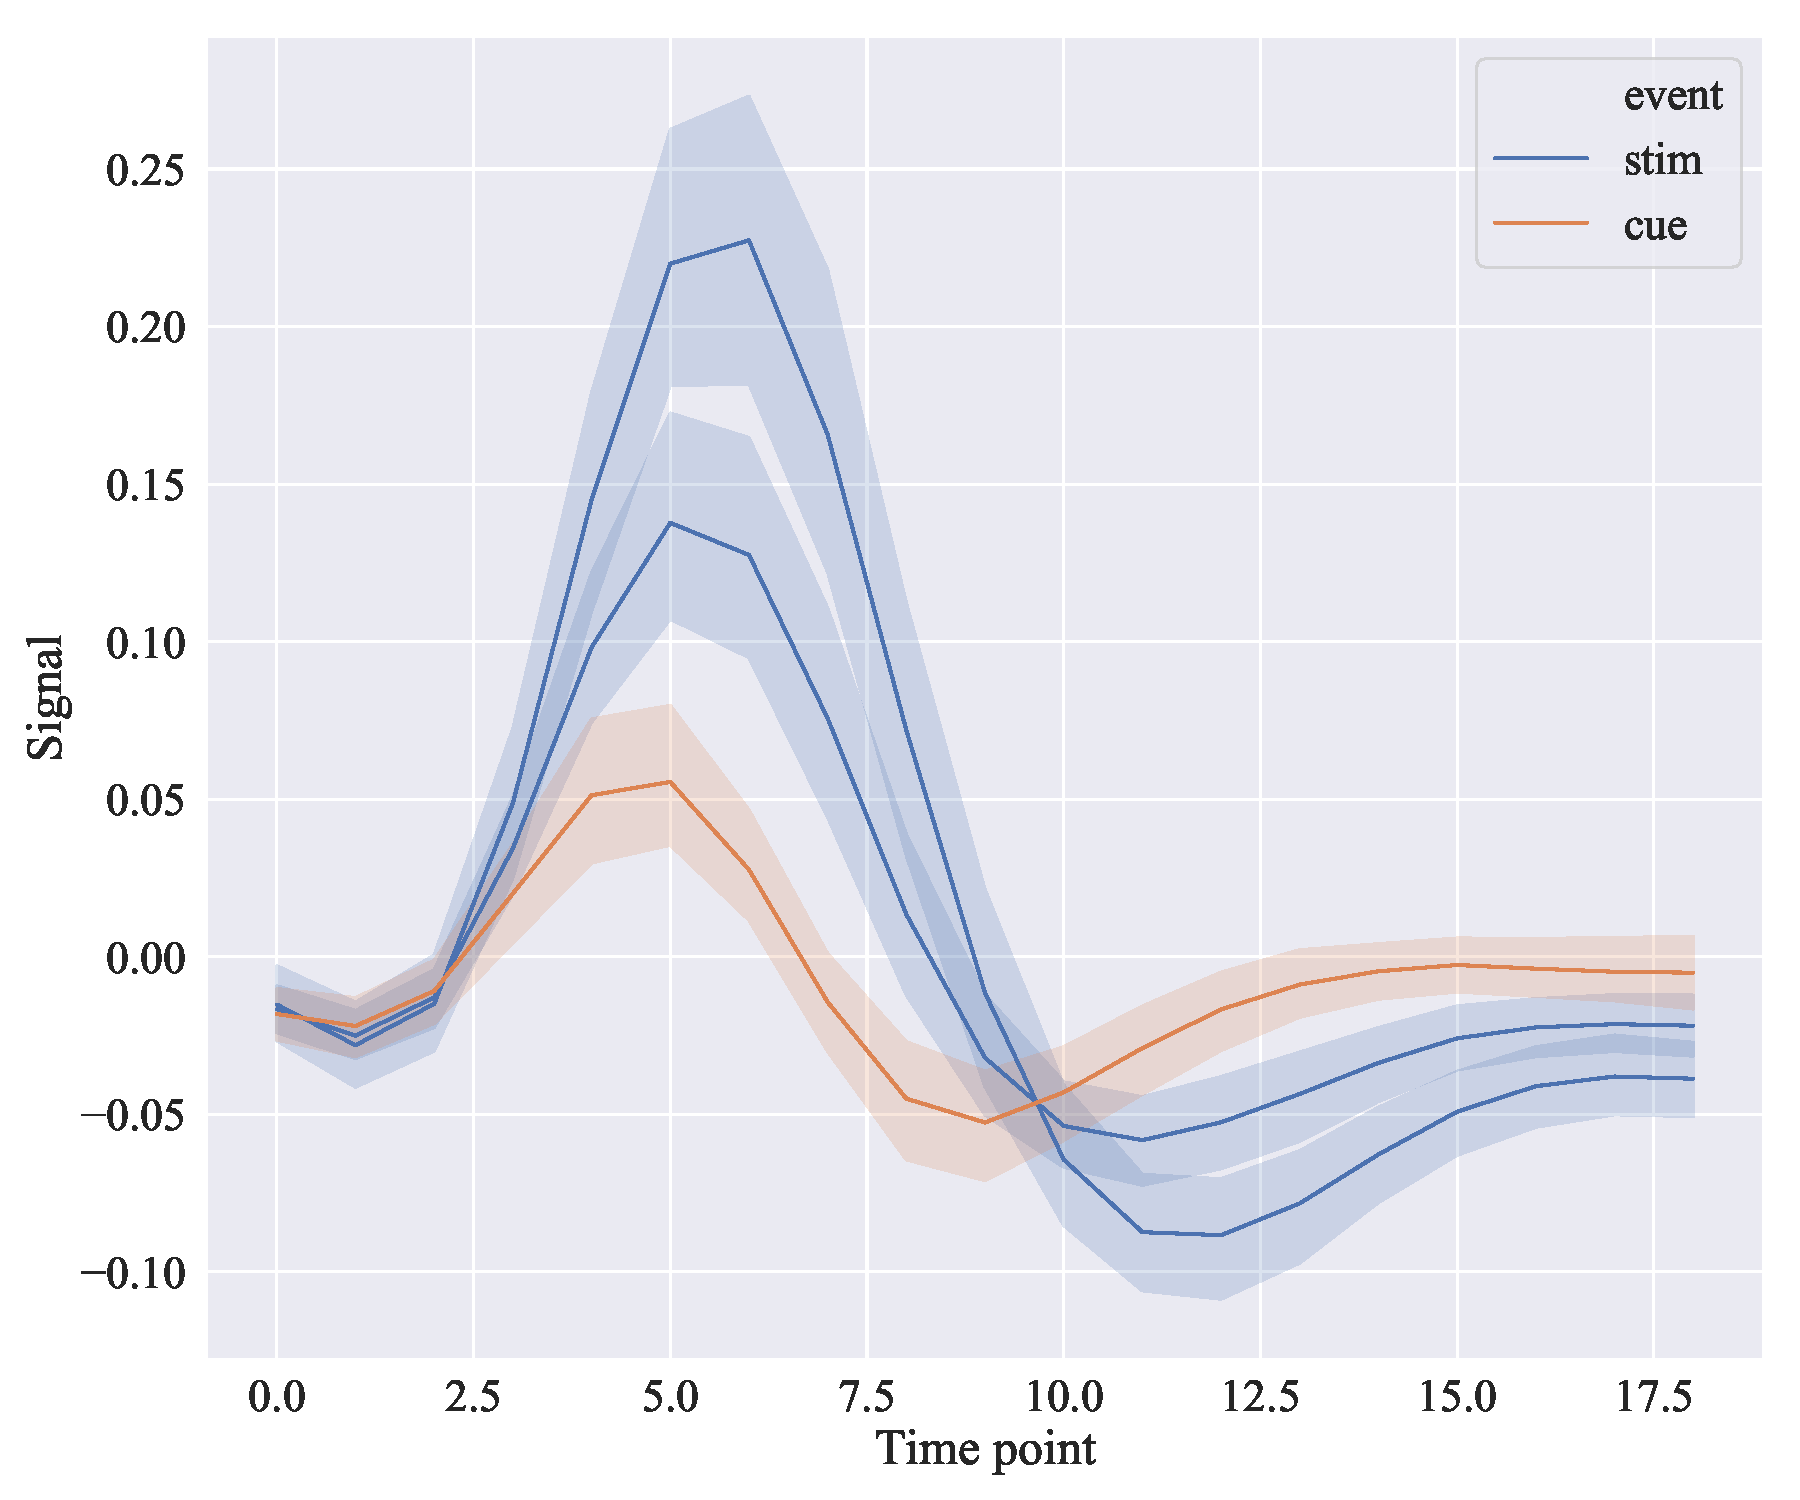
\includegraphics[width=0.8\textwidth]{fig_1.pdf} 
	% set figure caption
	\caption{An exemplary figure} 
	% set label for this figure so it can be refered in the text
	\label{fig_1} 
\end{figure} 
	\end{lstlisting}
	
	\begin{figure}[h!]
		\centering
		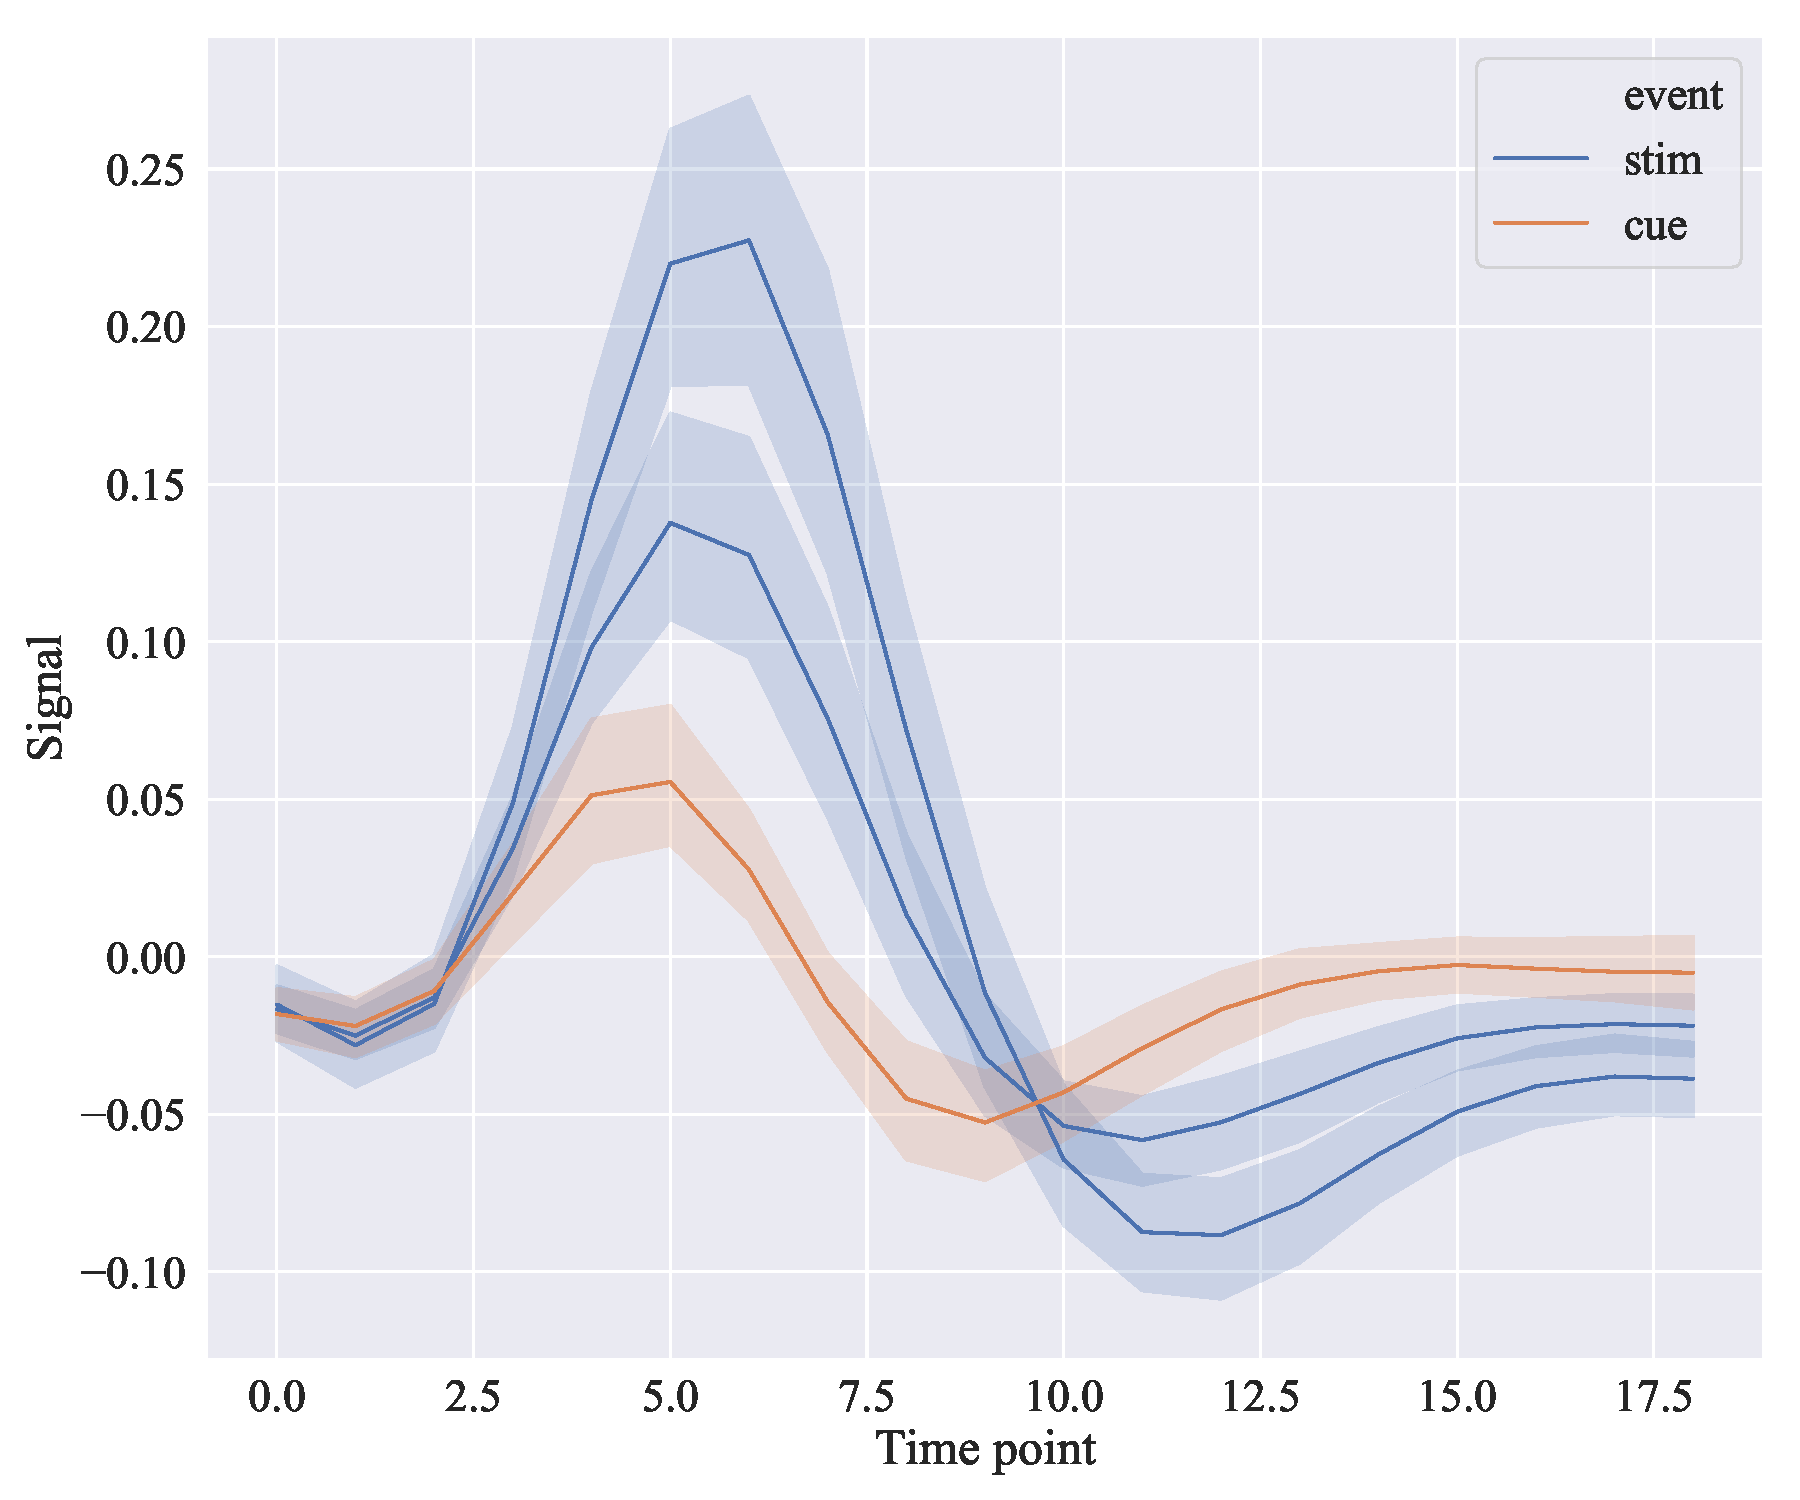
\includegraphics[width=0.8\textwidth]{fig_1.pdf} 
		\caption{An exemplary figure} 
		\label{fig_1} 
	\end{figure} 

	In this template, all exemplary figures are generated by matplotlib.pyplot library and scaled to wished size in the text. It should be however noticed, that due to the resizing process in \LaTeX, the font size set in original figures may be lost. Therefore, it is important to attempt different font size in your figures generated by software or programming languages. Another option is to utilize the {\color{blue}tikzpicture} package in \LaTeX, which can help to add text description of axes. An example of using {\color{blue}tikzpicture} package to obtain the same figure as Figure \ref{fig_1} is shown in Figure \ref{tikzpic}. You can compare this two figures and refer to the corresponding codes when necessary.

	\begin{figure}[h!]
		\centering
		\begin{tikzpicture}
		\node (img)  {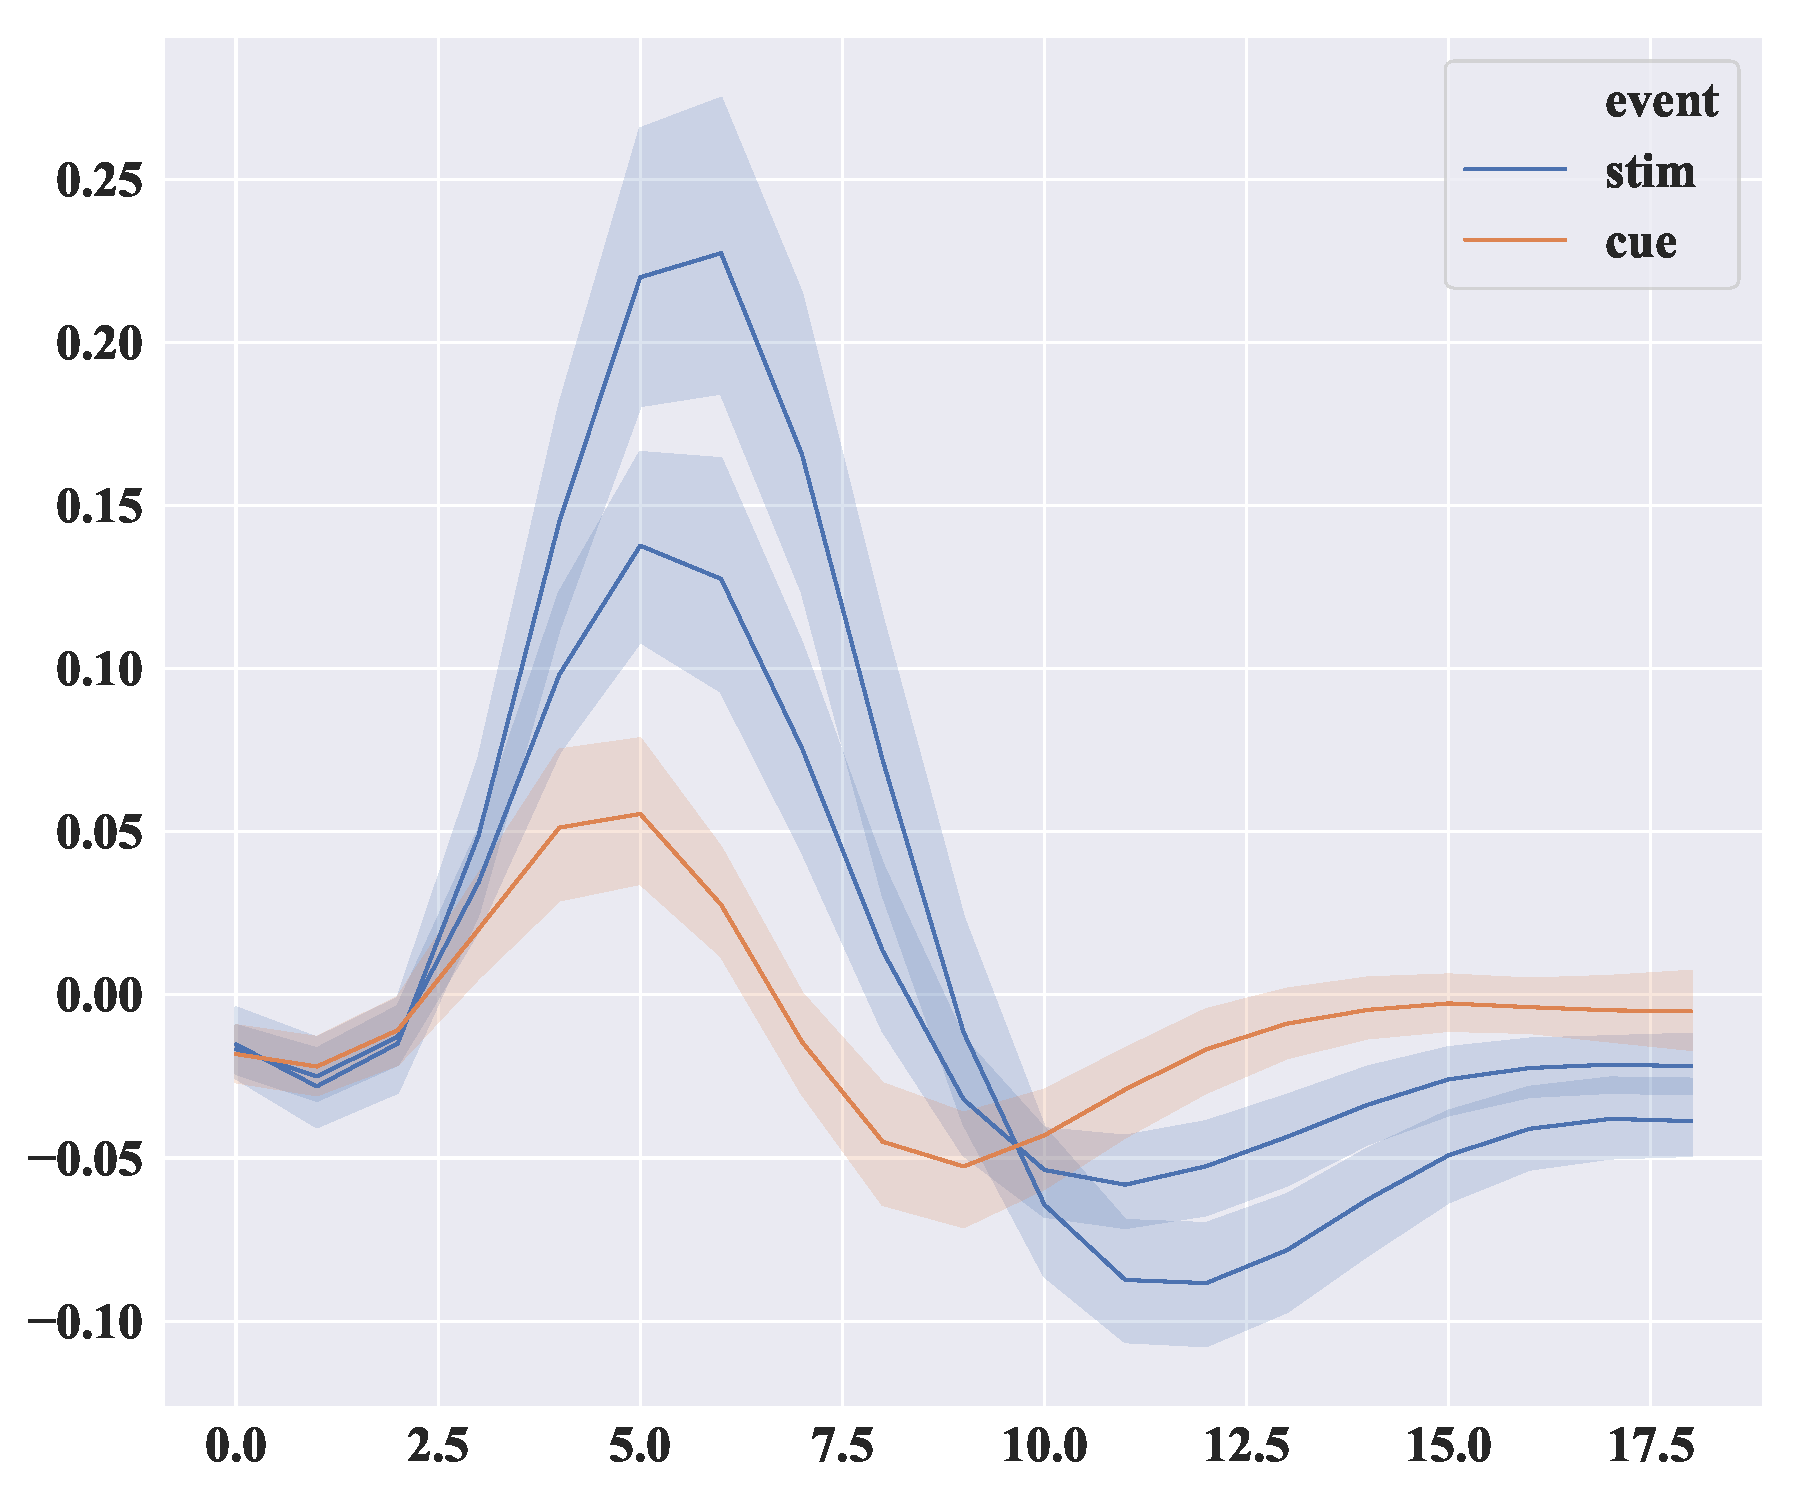
\includegraphics[width=0.8\textwidth]{fig_2.pdf}};
		\node[below=of img, node distance=0cm, yshift=1.2cm,font=\footnotesize] {Time point};
		\node[left=of img, node distance=0cm, rotate=90, anchor=center,yshift=-1cm,font=\footnotesize] {Signal};
		\end{tikzpicture}
		\caption{An example of tikzpicture}
		\label{tikzpic}
	\end{figure}

	Sometimes one need to insert multiple subplots at once. In \LaTeX~this can be realized by applying the {\color{blue}{\verb|\subfloat|}} environment. In Figure \ref{subfloats}, an example is shown, where four subfigures are included in one figure.
	
	\begin{figure}[h!]
		\centering
		\subfloat[Sub-1]{
			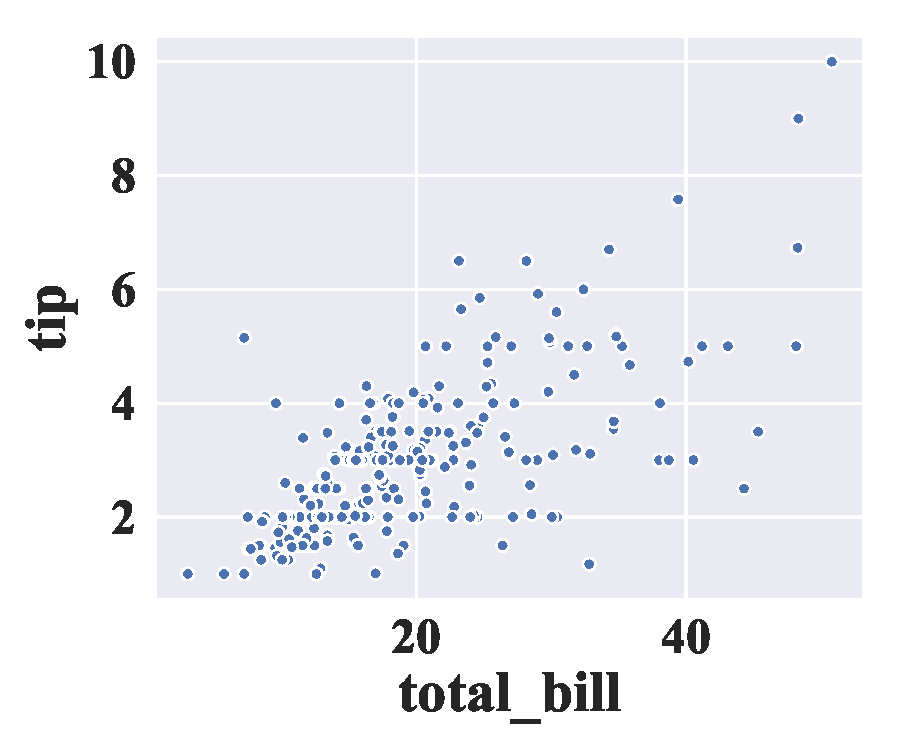
\includegraphics[width=0.4\textwidth]{sub_1.pdf}
			\label{sub_1}
		} \hspace{1cm}
		\subfloat[Sub-2]{
			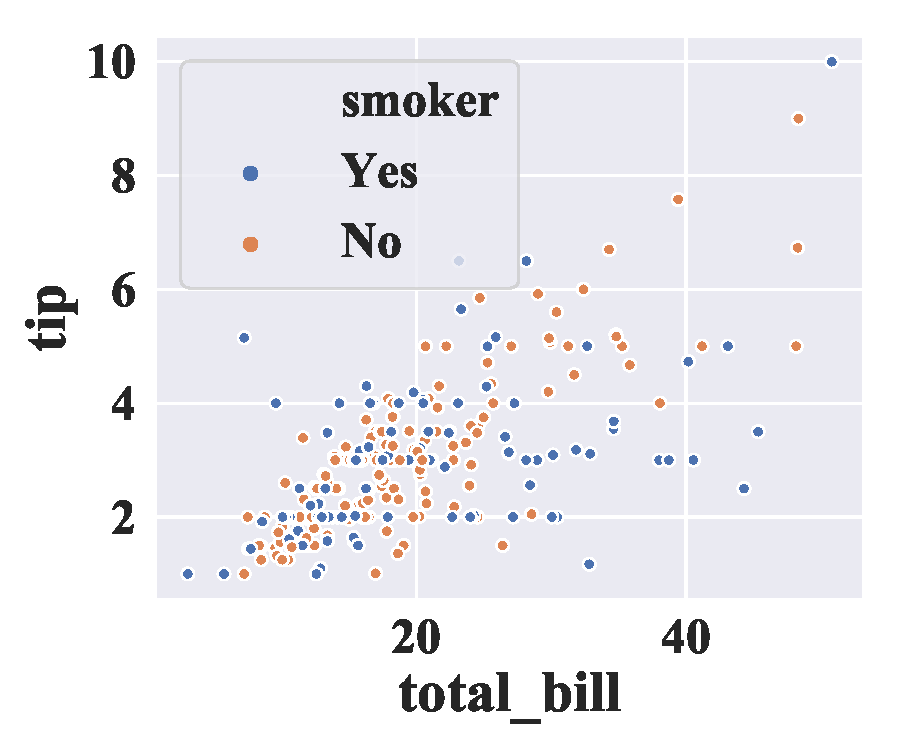
\includegraphics[width=0.4\textwidth]{sub_2.pdf}
			\label{sub_2}
		} \\
		\subfloat[Sub-3]{
			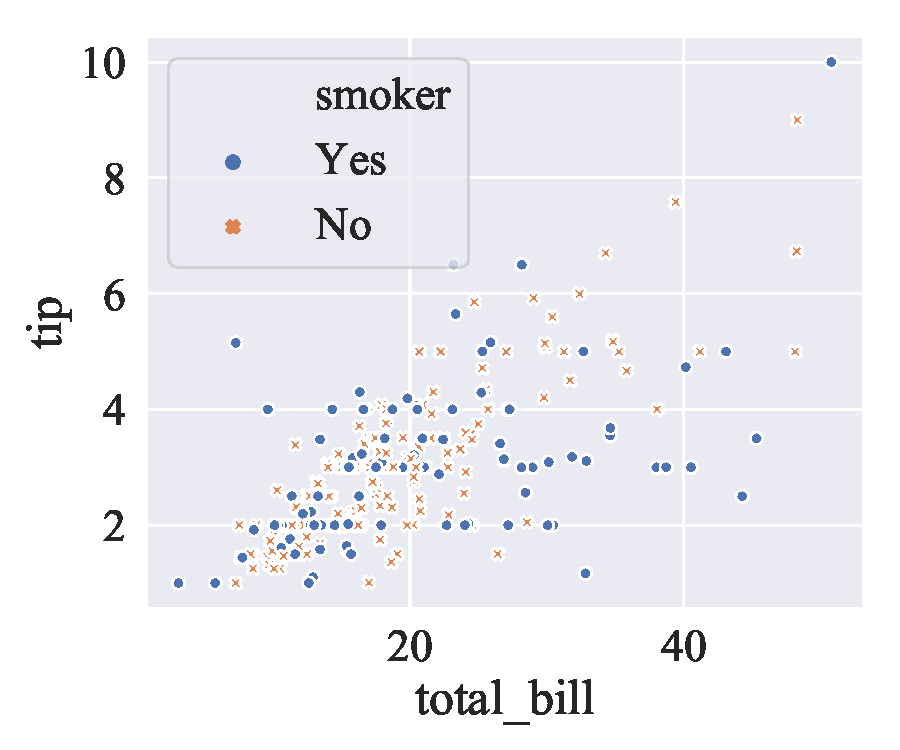
\includegraphics[width=0.4\textwidth]{sub_3.pdf}
			\label{sub_3}
		}
		\subfloat[Sub-4]{
			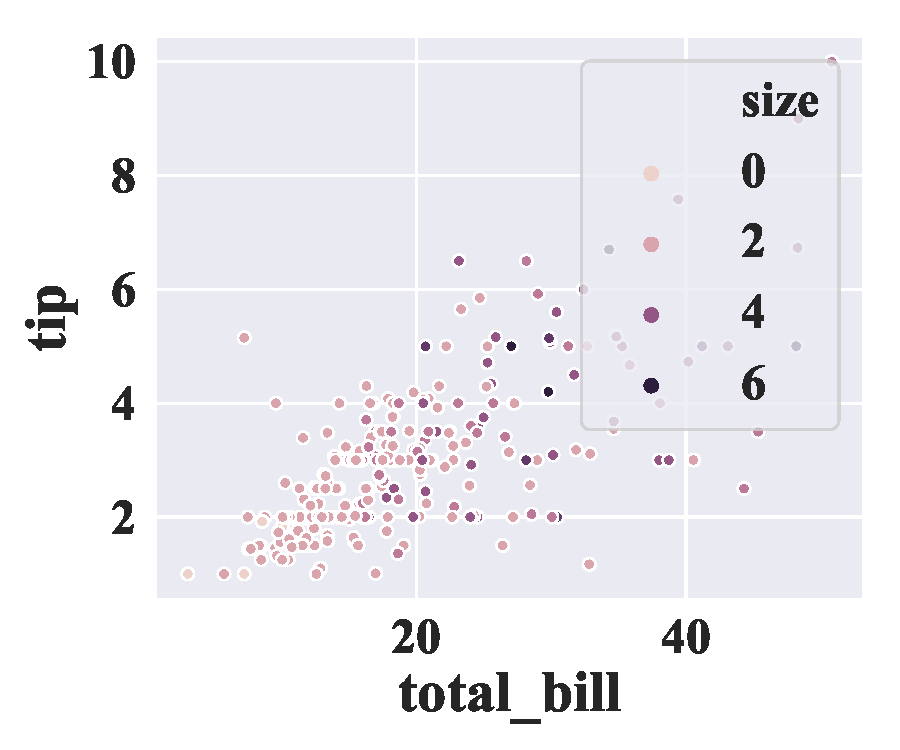
\includegraphics[width=0.4\textwidth]{sub_4.pdf}
			\label{sub_4}
		}
		\caption{Example of subfigures}\label{subfloats}
	\end{figure}

\newpage
	
\section{Inserting Tables}

	Table is another common element in scientific documents. \LaTeX~provides a large set of tools to customize tables. Some most common types and corresponding commands are shown in this section.
	
	The following code block shows a simple example to create a table. The parameter of command {\color{blue}{\verb|tabular|}} is aimed to set the number of columns, their delimiters and the alignment types. As shown in the exemplary codes, {\color{blue}{\texttt{{| l | c | r |}}}} creates a table with three columns and the ``|" symbols create vertical delimiters in the table. The letters are the definitions of alignment for each column, e.g. ``l" means left alignment, ``c" center and ``r" right. To add horizontal delimiters, just add {\color{blue}{\verb|\hline|}} before or after the entry of a row. 
	
	\begin{minipage}{\linewidth}
		\begin{lstlisting}
\begin{table}
	\centering
	\begin{tabular}{| l | c | r |}
		\hline
		Points per game & Rebounds per game & Assists per game \\ \hline
		7.6  & 1.9 & 1.3 \\ \hline
		15.4 & 3.1 & 2.5 \\ \hline
		19.9 & 5.3 & 3.8 \\ \hline
	\end{tabular}
\end{table}
		\end{lstlisting}
	\end{minipage}

	
	\begin{table}[h!]
		\centering
		\begin{tabular}{| l | c | r |}
			\hline
			Points per game & Rebounds per game & Assists per game \\ \hline
			7.6  & 1.9 & 1.3 \\ \hline
			15.4 & 3.1 & 2.5 \\ \hline
			19.9 & 5.3 & 3.8 \\ \hline
		\end{tabular}
		\caption{An exemplary table}
		\label{table_1}
	\end{table}
	
	Now the parameter {\color{blue}{\texttt{| l  c  r |}}} is used to format columns and some {\color{blue}{\verb|\hline|}} commands are removed, the output table is shown in Table \ref{table_2}.
	
	\begin{table}[h!]
		\centering
		\begin{tabular}{| l  c  r |}
			\hline
			Points per game & Rebounds per game & Assists per game \\ \hline
			7.6  & 1.9 & 1.3 \\ 
			15.4 & 3.1 & 2.5 \\
			19.9 & 5.3 & 3.8 \\ \hline 
		\end{tabular}
		\caption{Another exemplary table with fewer borders}
		\label{table_2}
	\end{table}

	It is sometimes necessary to merge several cells into one to make the table contents more evident. In \LaTeX~this function can be done by using {\color{blue}{\verb|\multicolumn{cols}{pos}{text}|}} or {\color{blue}{\verb|\multirow{number of rows}{width}{text}|}} commands. It should be noticed in Table \ref{table_4}, instead of using simply {\color{blue}{\verb|\hline|}}, {\color{blue}{\verb|\cline{2-3}|}} is used, which means add a horizontal border only from the 2nd to 3rd columns.
	
	\begin{table}[h!]
		\centering
		\begin{tabular}{| l | c | r |}
			\hline
			Points per game & Rebounds per game & Assists per game \\ \hline
			\multicolumn{2}{| c |}{N/A} & 1.3 \\ \hline 
			15.4 & 3.1 & 2.5 \\
			19.9 & 5.3 & 3.8 \\ \hline 
		\end{tabular}
		\caption{Exemplary table with horizontally merged cells}
		\label{table_3}
	\end{table}

	\begin{table}[h!]
		\centering
		\begin{tabular}{| l | c | r |}
			\hline
			Points per game & Rebounds per game & Assists per game \\ \hline
			\multirow{2}*{N/A} & 1.9 & 1.3 \\ \cline{2-3} 
			& 3.1 & 2.5 \\ \hline
			19.9 & 5.3 & 3.8 \\ \hline 
		\end{tabular}
		\caption{Exemplary table with vertically merged cells}
		\label{table_4}
	\end{table}

	In chapter 1 the color function in \LaTeX~has already been introduced. The colors can be set as the background color with {\color{blue}{\verb|\rowcolor|}} or {\color{blue}{\verb|\rowcolors|}} commands. The first one is used to set color for a single row, while the second one can automatically alternate the row color as shown in Figure \ref{table_5}, where the color is defined before and the title is set to 60\% and the other rows alternates between 20\% and 40\%.
	
	\definecolor{lal-g}{RGB}{253, 185, 39}
	\definecolor{lal-p}{RGB}{85, 37, 130}
	\definecolor{lal-b}{RGB}{6, 25, 34}
	
	\begin{table}[h!]
		\centering
		\rowcolors{1}{new-color!20}{new-color!10}
		\begin{tabular}{ l  c  r }
			\rowcolor{new-color!60}
			Points per game & Rebounds per game & Assists per game \\ 
			7.6  & 1.9 & 1.3 \\ 
			15.4 & 3.1 & 2.5 \\
			19.9 & 5.3 & 3.8 \\ 
			22.5 & 6.3 & 4.9 \\
			25.2 & 5.5 & 5.5 \\ 
		\end{tabular}
		\caption{Exemplary table with two colors}
		\label{table_5}
	\end{table}  

	Sometimes the description or content in a table cell is too long, with {\color{blue}\textbf{tabular}} environment the cell width will always fit the input text length (as shown in Table \ref{table_6}). To wrap the text inside a cell, you can use multiple methods, here in this template the environment or package {\color{blue}\textbf{tabularx}} is introduced, which original aims to make tables with fixed cell width.
	
	To use {\color{blue}\textbf{tabularx}}, you should enter an option for the table width, so that the generated table will always have the width as you set. It has also an extra description {\color{blue}X} for column format is defined, which can be used to divide the set width and make all columns with X-type the same width, you can refer to Table \ref{table_7} and the corresponding source code.
	
	\begin{table}[h!]
		\centering
		\rowcolors{1}{lal-p!40}{lal-g!40}
		\begin{tabular}{| c  c  c  c  c |}
			\rowcolor{lal-p!60}
			\hline
			Season  & Minutes per game  & Points per game  & Rebounds per game & Assists per game \\
			1996–97 & 15.5 & 7.6  & 1.9 & 1.3 \\
			1997–98	& 26.0 & 15.4 &	3.1	& 2.5 \\
			1998–99	& 37.9 & 19.9 &	5.3 & 3.8 \\
			1999–00	& 38.2 & 22.5 &	6.3	& 4.9 \\
			2001–02 & 38.3 & 25.2 &	5.5	& 5.5 \\
			2002–03 & 41.5 & 30.0 & 6.9 & 5.9 \\
			\hline
		\end{tabular}
		\caption{Table width exceeds the text width}
		\label{table_6}
	\end{table}  
	
	\begin{table}
		\centering
		\rowcolors{5}{lal-p!40}{lal-g!40}
		\begin{tabularx}{0.9\textwidth}{| X | X | X | X | X |}
			\rowcolor{lal-p!60}
			\hline
			Season  & Minutes per game  & Points per game  & Rebounds per game & Assists per game \\
			1996–97 & 15.5 & 7.6  & 1.9 & 1.3 \\
			1997–98	& 26.0 & 15.4 &	3.1	& 2.5 \\
			1998–99	& 37.9 & 19.9 &	5.3 & 3.8 \\
			1999–00	& 38.2 & 22.5 &	6.3	& 4.9 \\
			2001–02 & 38.3 & 25.2 &	5.5	& 5.5 \\
			2002–03 & 41.5 & 30.0 & 6.9 & 5.9 \\
			\hline
		\end{tabularx}
		\caption{An exemplary tabularx}
		\label{table_7}
	\end{table}

	It should be noticed, the X-type in {\color{blue}\textbf{tabularx}} set the alignment to left side of the cells. To center the contents in these cells, one can define a new Y-type with the command {\color{blue}{\verb|\newcolumntype{Y}{>{\centering\arraybackslash}X}|}}. Now set all X-type columns in Table \ref{table_7} as Y-type, Table \ref{table_8} can be obtained.
	
	\newcolumntype{Y}{>{\centering\arraybackslash}X}

	\begin{table}
	\centering
	\rowcolors{5}{lal-p!40}{lal-g!40}
		\begin{tabularx}{0.9\textwidth}{| Y | Y | Y | Y | Y |}
			\rowcolor{lal-p!60}
			\hline
			Season  & Minutes per game  & Points per game  & Rebounds per game & Assists per game \\
			1996–97 & 15.5 & 7.6  & 1.9 & 1.3 \\
			1997–98	& 26.0 & 15.4 &	3.1	& 2.5 \\
			1998–99	& 37.9 & 19.9 &	5.3 & 3.8 \\
			1999–00	& 38.2 & 22.5 &	6.3	& 4.9 \\
			2001–02 & 38.3 & 25.2 &	5.5	& 5.5 \\
			2002–03 & 41.5 & 30.0 & 6.9 & 5.9 \\
			\hline
		\end{tabularx}
		\caption{Center contents in a tabularx}
		\label{table_8}
	\end{table}
